\mysection{РАЗРАБОТКА АРХИТЕКТУРЫ ПРОГРАММЫ}
\
\subsection{Требования к реализуемой программе}
\

Требования к программам и системам можно разделить на функциональные и нефункциональные. Функциональные требования позволяют обозначить функционал, которым должна обладать программа для удовлетворения просьб заказчика. Нефункциональные требования — это дополнительные атрибуты качества, которые важны для разработчика и заказчика.

К разрабатываемой программы были поставлены следующие функциональные требования:

\begin{itemize}
  \item Программа должна иметь функционал для сохранения и загрузки обученной модели;
  \item Программа не должна находить связь, если в запросе был указан товар, который не существует в базе клиента;
  \item Предсказания должны осуществляться с точностью более 90\%;
  \item Время ответа классификатора не должно превышать 0.1 с.
\end{itemize}

\
Нефункциональные требования:
\begin{itemize}
  \item Программа должна иметь API для возможности интеграции в приложение.
\end{itemize}

\newpage

\subsection{Проектирование архитектуры}
\

Для разработки программы была выбрана модульная архитектура. Модульная архитектура — архитектура, при которой программа организована как совокупность независимых друг от друга блоков, структура и поведение которых подчиняются определенным правилам. Использование такой архитектуры позволяет упростить тестирование и масштабирование, так как каждый модуль имеет строго определенные задачи, которые можно дополнять и тестировать отдельно от остальных модулей.

Использование данной архитектуры позволило разбить программу на три фрагмента: обучение, классификация, API. Структура программы представлена на рисунке 2.1.

\


  \begin{figure}[h!]
    \centering
    \setlength{\fboxsep}{5pt}
    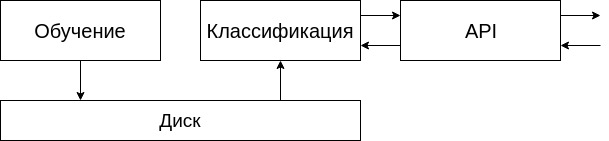
\includegraphics[width=.9\textwidth]{img/module-structure}
    \vspace*{6pt}
    \caption{Структура программы}\label{fig:project-tree}
  \end{figure}


Одной из основных задач разработки является выбор языка программирования. Для реализации программы был выбран Python. Python — высокоуровневый язык программирования общего назначения. Отличительной чертой Python является минималистичность сиктаксиса, что повышает произвоидельность и скорость разработчика, а также читаемость кода.\cite{Python} Простота Python в совокупности с большим количеством библиотек как для работы с данными, так и для машинного обучения делают его очень популярным инструментом для математических расчетов и задач, связанных с анализом и машинным обучением.

Модули программы:

\begin{itemize}
  \item Процесс обучения представлен модулем на языке Python, взаимодействие с которым происходит через методы класса с помощью интерпретатора данного языка через командную строку. Используется для построения и обучения классификатора. Результатом работы явлется запись на диск файла обученного классификатора и вспомогательных файлов, которые в последствии используются модулем классификации;
  \item Модуль классификации в качестве входных данных принимает документ, класс которого требуетс определить, а также загружает с диска файл классификатора. Выходными данными является метка, которую определил классификатор. Взаимодействие с модулем происходит через методы класса с помощью интерпретатора Python через командную строку напрямую или же через API;
  \item API — средство для общения клиента с обученным классификатором с целью получения предсказания. Взаимодействие происходит через HTTP-запросы, входные данные — это документ, требующий классификации, а выходные — класс.
\end{itemize}

\newpage
\subsubsection{Проектирование модуля обучения}
\

Для подготовки данных, построения и обучения классификатора была использована библиотека \textbf{Scikit-learn}.\cite{Scikit} Это наиболее популярная бесплатная библиотека для машинного обучения на языке Python. Она реализует различные алгоритмы классификации, регрессии и кластеризации, включая машины опорных векторов, случайные леса, повышение градиента, k-средних и DBSCAN, и предназначена для взаимодействия с математическими библиотеками NumPy и SciPy. В ее возможности также входит преобразование данных, извлечение признаков, нормализация, удаление шумовых слов.

\textbf{NumPy} — библиотека с открытым исходным кодом для языка программирования Python, основными возможностями которой являются поддержка многомерных массивов и поддержка высокоуровневых математических функций, предназначенных для работы с многомерными массивами\cite{NumPy}.

Еще одним инструментом, использующимся совместно с Scikit-learn является библиотека для обработки и анализа данных \textbf{pandas}, которая строится поверх NumPy. Представляет специальные структуры данных для манипулирования индексированными массивами двумерных данных, которые были использованы при загрузке и подготовке корпуса обучающих данных\cite{pandas}.

\

  \begin{figure}[h!]
    \centering
    \setlength{\fboxsep}{5pt}
    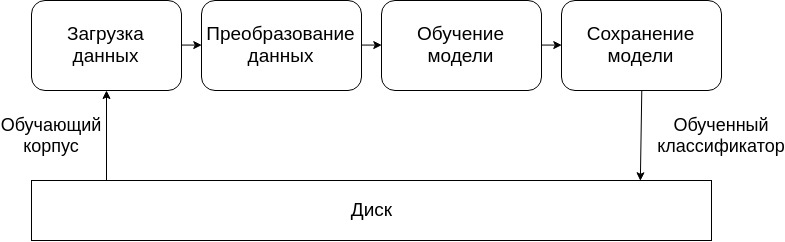
\includegraphics[width=.99\textwidth]{img/learn-module}
    \vspace*{6pt}
    \caption{Структура модуля обучения}\label{fig:project-tree}
  \end{figure}

 \

Для сохранения и загрузки файлов обученного классификатора была использована библиотека Joblib. \textbf{Joblib} — это набор инструментов для облегченной конвейерной обработки в Python. В частности, инструменты дампа и загрузки данных\cite{Joblib}.

Структура модуля обучения представлена на рисунке 2.2. Данный модуль с помощью описанных выше библиотек решает ряд задач: загрузку обучающих данных из файла, подготовку данных, извлечение признаков, нормализацию, построение и обучение классификатора, сохранение классификатора для дальнейшего использования. Этот модуль работает независимо от остальных модулей программы и используется только для создания обученной модели, поэтому взаимодействие с ним происходит с помощью интерфейса командной строки через интерпретатор Python. 

\newpage
\subsubsection{Проектирование модуля классификации}
\

Преобразование данных перед классификацией происходит так же, как и в обучающем модуле, посредством библиотеки Scikit-learn. Входными данными является текстовый документ, который необходимо классифицировать. Он представляется в виде вектора, после чего передается классификатору. Результатом классификации является метка класса, к которому относится входной документ, представленная в форме строки.

\

  \begin{figure}[h!]
    \centering
    \setlength{\fboxsep}{5pt}
    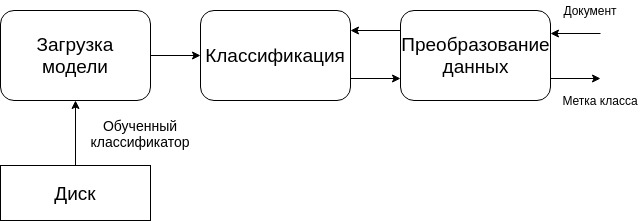
\includegraphics[width=.99\textwidth]{img/classification-module}
    \vspace*{6pt}
    \caption{Структура модуля обучения}\label{fig:project-tree}
  \end{figure}


Структура модуя классификации представлена на рисунке 2.3. Чтобы осуществить классификацию, необходимо сначала загрузить обученный классификатор и вспомогательные файлы (модели для преобразования входных данных) с диска. После загрузки модели классификатора с ним осуществляется взаимодействие с помощью интерфейса командной строки через интерпретатор Python или через модуль API.

\newpage
\subsubsection{Проектирование API}
\

Для соответствия программы нефункциональному требованию о возможности интеграции в другое приложение был разработан модуль API. Он представляет из себя веб-сервер, созданный с использованием Flask. \textbf{Flask} — фреймворк для создания веб-приложений на языке программирования Python, относится к категории микрофреймворков — минималистичных каркасов веб-приложений, предоставляющих лишь самые базовые возможности\cite{Flask}. Этот фреймворк в рамках данной работы был выбран для создания API из-за его минималистичности, простоты использования и запуска. 

Взаимодействие клиента с API произходит через HTTP-запросы. HTTP — протокол прикладного уровня передачи данных, в настоящий момент используется для передачи произвольных данных. Основой HTTP является технология «клиент-сервер», то есть предполагается существование:

\begin{itemize}
  \item Клиентов, которые инициируют соединение и посылают запрос;
  \item Серверов, которые ожидают соединения и запроса, производят необходимые действия и возвращают клиенту сообщение с результатом. 
\end{itemize}

Серверная часть API извлекает требующий классификации документ из запроса, передает его модулю классификации, и, получив ответ классификатора, возвращает этот ответ клиенту посредсвом HTTP.
\newpage